\section{Related Work}\label{sec:ch6:related} 
Fujieda et.\ al.\ use a DWT in combination with a
CNN to do texture classification and image annotation 
\cite{fujieda_wavelet_2017, fujieda_wavelet_2018}. In particular, they take a
multiscale wavelet transform of the input image, combine the actviations at each
scale independently with learned weights, and feed these back into the network
where the activation resolution size matches the subband resolution. The
architecture block diagram is shown in \autoref{fig:ch6:fujieda}, taken from the
original paper.  This work found that their dubbed `Wavelet-CNN' could
outperform competetive non wavelet based CNNs on both texture classification and
image annotation.

\begin{figure}[bt]
  \centering
  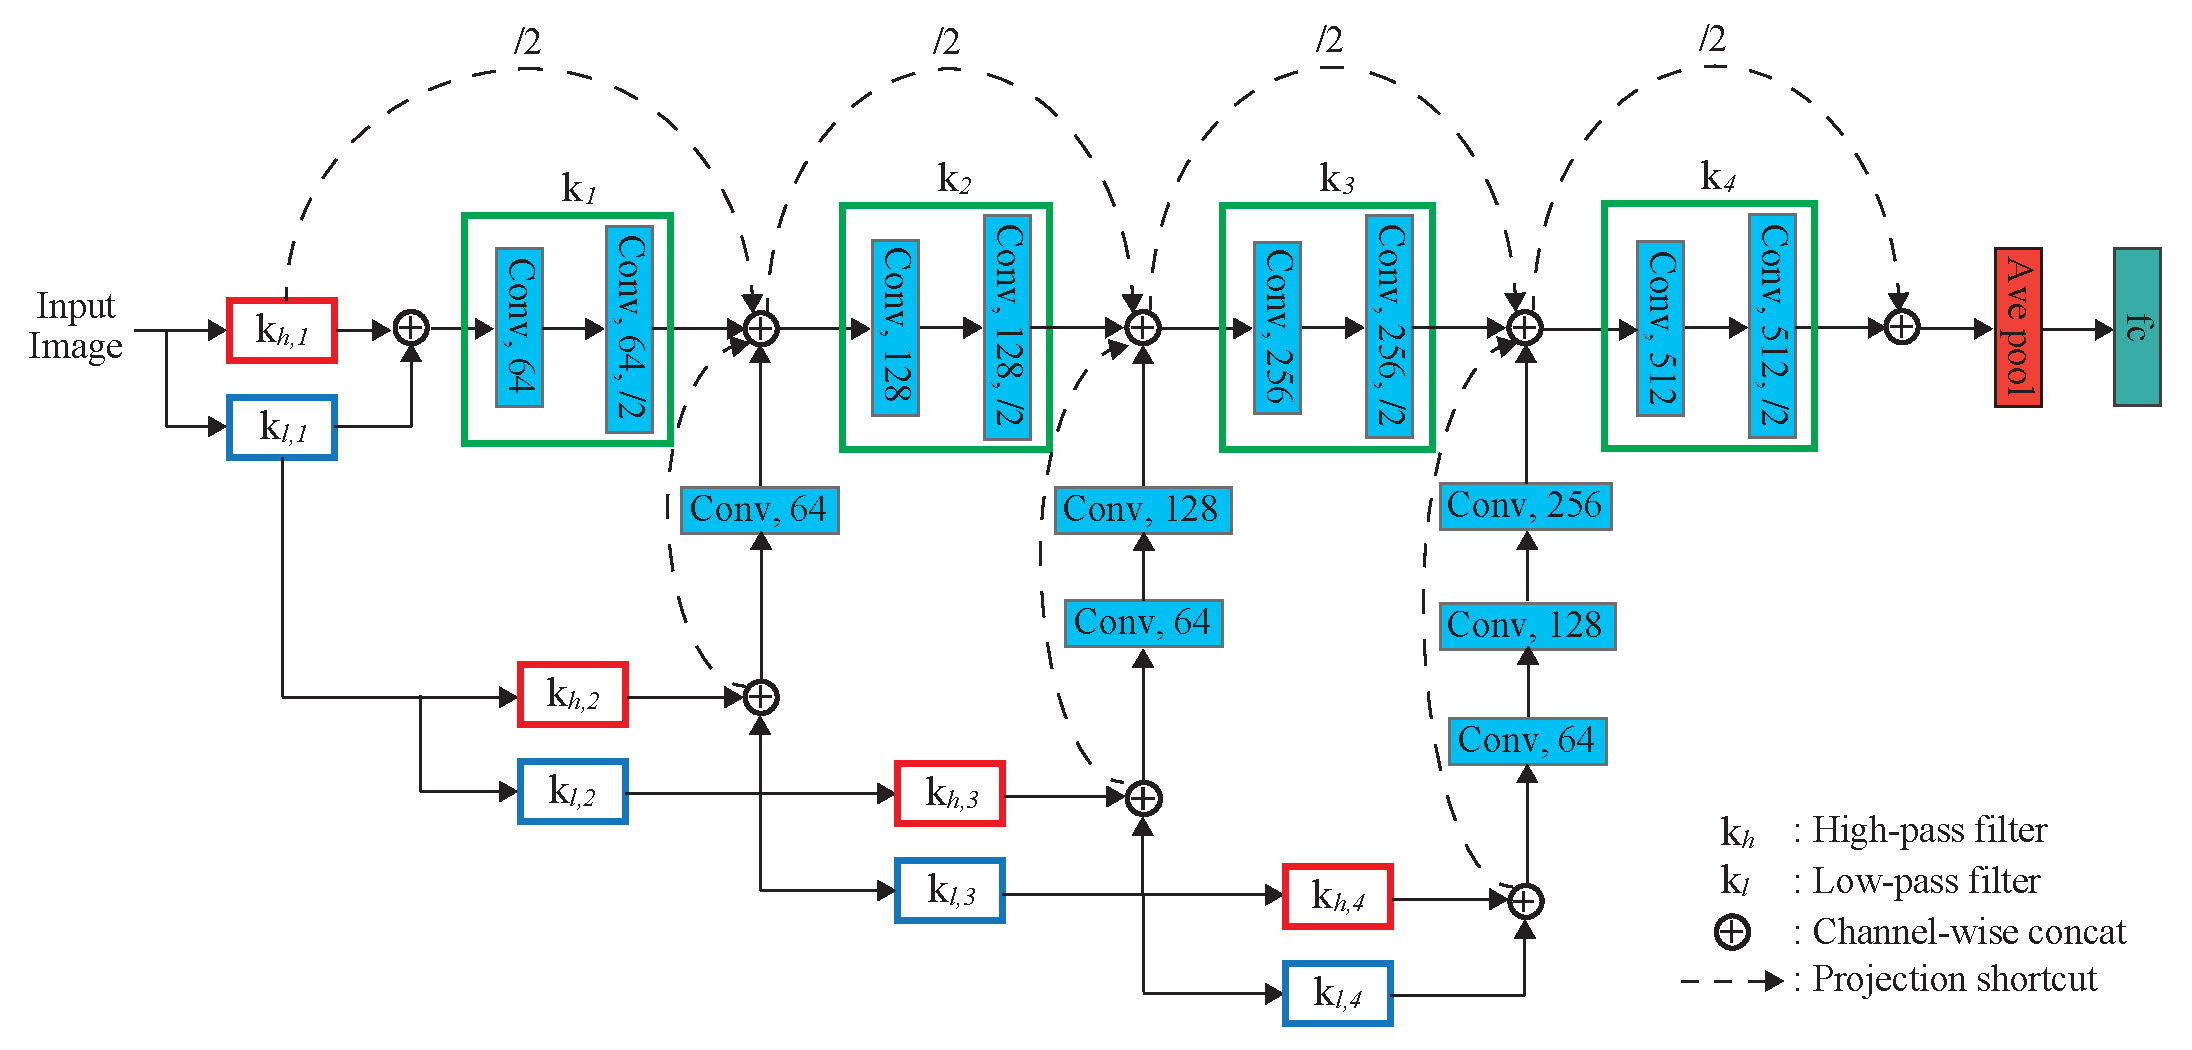
\includegraphics[width=\textwidth]{\imgpath/wavelet_CNN_3.pdf}
  \mycaption{Architecture using the DWT as a frontend to a CNN}{Figure 1 from
  \cite{fujieda_wavelet_2018}. Fujieda et.\ al.\ take a multiscale wavelet
  decomposition of the input before passing the input through a standard
  CNN\@. They learn convolutional layers independently on each subband and feed
  these back into the network at different depths, where the resolution of the
  subband and the network activations match.}
  \label{fig:ch6:fujieda}
\end{figure}

Several works also use wavelets in deep neural networks for super-resolution
\cite{guo_deep_2017} and for adding detail back into dense pixel-wise
segmentation tasks \cite{ma_detailed_2018}. These typically save wavelet
coefficients and use them for the reconstruction phase.

In \cite{rippel_spectral_2015}, \citeauthor{rippel_spectral_2015}
parameterize filters in the DFT domain. Rather than having a pixel domain filter
$\vec{w} \in \reals[F\x C\x K\x K]$, they learn a set of fourier coefficients
$\hat{\vec{w}} \in \complexes[F\x C\x K \x \ceil{K/2}]$
(the reduced spatial size is a result of enforcing that the inverse DFT of their
filter to be real, so the parameterization is symmetric). On the forward pass of
the neural network, they take the inverse DFT of $\hat{\vec{w}}$ to obtain
$\vec{w}$ and then convolve this with the input $\vec{x}$ as a normal CNN
would do.\footnote{The convolution may be done by taking both the image and
filter back into the fourier space but this is typically decided by the
framework, which selects the optimal convolution strategy for the filter and
input size. Note that there is not necessarily a saving to be gained by
enforcing it to do convolution by product of FFTs, as the FFT size needed for
the filter will likely be larger than $K\x K$, which would require resampling
the coefficients}. 

Note that an important point should be laboured about reparameterizing filters
in either the wavelet or Fourier domains: any invertible linear
transform of the parameter space will not change the updates if a linear
optimization scheme is used (for example standard gradient descent, or SGD with momentum)\footnote{This fact 
is something that \citeauthor{rippel_spectral_2015} briefly allude to, but do not make clear}.
This is proved in \autoref{app:ch6:invertible}.  
We make this point clear as a natural extension to continue the work
in \cite{rippel_spectral_2015} would be to parameterize filters in the wavelet domain,
taking inverse transforms to the pixel domain and doing normal convolution. 

The work presented in this chapter does not learn wavelet coefficients 
for convolutional filters to be applied in the pixel domain, rather we learn wavelet filters 
\emph{and} do convolution in the wavelet domain too.

\section{Background and Notation}
We make use of the 2-D $Z$-transform to simplify our analysis:
%
\begin{equation}
  X(\zz) = \sum_{n_1}\sum_{n_2} x[n_1, n_2]z_1^{-n_1}z_2^{-n_2} =
  \sum_{\nn}x[\nn]\zz^{-\nn}
\end{equation}
%
As we are working with three dimensional arrays (two spatial and one channel) but are
only doing convolution in two, we introduce a slightly modified 2-D $Z$-transform
which includes the channel index, $c$:
%
\begin{equation}
  X(c, \zz) = \sum_{n_1}\sum_{n_2} x[c, n_1, n_2]z_1^{-n_1}z_2^{-n_2} =
  \sum_{\nn}x[c, \nn]\zz^{-\nn} \label{eq:ch6:ztransform}
\end{equation}
We then define the product of these new $Z$-transform signals to be the
channel-wise convolution. E.g. for the 3-D filter $h[c, \nn]$ with $Z$-transform
$H(c, \zz)$ and the the 3-D signal $x[c, \nn]$ with $Z$-transform $X(c, \zz)$,
let us call the product of the two $Z$-transforms:
\begin{equation}
  H(c, \zz)X(c, \zz) = \sum_{\nn}\left(\sum_{\bmu{k}}h[c, \nn-\bmu{k}]x[c, \bmu{k}]\right)\zz^{-\nn} \label{eq:ch6:zproduct}
\end{equation}
%
Recall from \autoref{sec:ch2:conv_layers} that a typical convolutional
layer in a standard CNN gets the next layer's output in a two-step process:
%
\begin{align} 
  \cnndlact{y}{l+1}{f}{\nn} &= \sum_{c=0}^{C_l - 1} \cnndlact{x}{l}{c}{\nn} \conv \cnndfilt{l}{f}{c}{\nn}
    \label{eq:ch6:conv}\\
    \cnndlact{x}{l+1}{f}{\nn} & =  \sigma \left( \cnndlact{y}{l+1}{f}{\nn} \right) \label{eq:ch6:nonlin}
\end{align}
%
If we define the nonlinearity $\sigma_z$ to be the action of $\sigma$ to each
$z$-coefficient in the polynomial $Y(c, \zz)$, then we can rewrite
\eqref{eq:ch6:conv} and \eqref{eq:ch6:nonlin} as:
%
\begin{align}
  \cnnlact{Y}{l+1}{f}{\zz} &= \sum_{c=0}^{C_l - 1} \cnnlact{X}{l}{c}{\zz} H_f^{(l)}(c, \zz) \\
  \cnnlact{X}{l+1}{f}{\zz} &= \sigma_z(\cnnlact{Y}{l+1}{f}{\zz})
\end{align}
%
\subsection{$\DTCWT$ Notation}
For this chapter, we will work with lots of $\DTCWT$ coefficients so we define
some slightly new notation here.

A $J$ scale 2-D $\DTCWT$ gives $6J+1$ coefficients, 6 sets of complex
bandpass coefficients for each scale (representing the oriented bands from 15 to 165
degrees) and 1 set of real lowpass ($lp$) coefficients. 
\begin{equation}
  \DTCWT_J(x) = \{ u_{lp}, u_{j,k} \}_{1\leq j\leq J, 1\leq k\leq 6}
  \label{eq:ch6:dtcwt_coeffs}
\end{equation}

Each of these coefficients then has size:
%
\begin{eqnarray}
  u_{lp} &\in & \reals[N\x C\x \frac{H}{2^{J-1}} \x \frac{W}{2^{J-1}}] \\
  u_{j,k} &\in & \complexes[N\x C\x \frac{H}{2^{J}}\x \frac{W}{2^{J}}]
\end{eqnarray}
%
Note that the lowpass coefficients are twice as large as in a fully decimated
transform, a feature of the redundancy of the $\DTCWT$ and the fact that the
lowpass coefficients are most conveniently represented as purely real values,
whereas the bandpass ones are most conveniently complex in \eqref{eq:ch6:dtcwt_coeffs}.

If we ever want to refer to all the subbands at a given scale, we will
drop the $k$ subscript and call them $u_j$. Likewise, $u$ refers to the whole
set of $\DTCWT$ coefficients.


